%%
%% This is file `example/ch_intro.tex',
%% generated with the docstrip utility.
%%
%% The original source files were:
%%
%% install/buptgraduatethesis.dtx  (with options: `ch-intro')
%% 
%% This file is a part of the example of BUPTGraduateThesis.
%% 

\chapter{绪论}
\section{研究背景及意义}
软件定义网络(Software Defined Networking,简称SDN)是一种时下热门的网络架构,在这种网络架构中,网络控制平面与转发平面分离,完成了对网络的集中控制,并且网络是直接可编程,用户可以根据自己的需求,定制化网络业务。以前,网络的控制权与网络设备是紧密捆绑的,现在控制权的迁移使得底层构架能够抽象出来,各种应用和网络服务因此能将网络当作一个逻辑或虚拟实体。

通过应用SDN,除了网络的设计和操作变得简化,网络设备也得到简化,这些设备无需理解或处理成千上万的协议,只需要接受SDN控制器的指令即可。利用集中控制,网络管理员可以实时改变网络的行为,并且在几小时或几天内就可以部署新的应用和网络服务。

网络虚拟化是一种将底层网络中的硬件以及配套的软件资源进行整合,形成统一管理实体的技术,通过虚拟网络资源到物理网络资源的映射,使得多个逻辑虚拟网络共享底层物理网络基础设施。网络虚拟化技术是当今网络革新的重要技术之一。从概念上,网络虚拟化与SDN是互相独立的,但随着近几年网络技术的发展与融合,二者之间的联系变得越来越紧密,SDN的技术相关专题常会提及网络虚拟化技术,网络虚拟化问题的研究也时常会运用到SDN的概念,可见基于SDN的网络虚拟化技术已经成为网络技术研究领域的一个专门课题。

OpenStack是一个开源的云计算管理平台项目,旨在为公共及私有云的建设与管理提供软件的开源项目,主要提供计算、存储、网络服务。OpenStack支持几乎所有类型的云环境,项目目标是提供实施简单、可大规模扩展、丰富、标准统一的云计算管理平台。OpenStack通过各种互补的服务提供了基础设施即服务(IaaS)的解决方案,每个服务提供API以进行集成。

在现有OpenStack云平台中,租户网络的创建与隔离仅限于服务器内部,对云平台服务器外围交换机(以下统称为数据中心网络)的管控一直是空白点,如果租户想要与其他服务器通信,服务器内部的vswitch需要对数据包进行Tumnel(VLAN或者GRE)操作,但是该操作有很多弊端,吞吐量偏低,延时偏大,抖动比较大,盛科为了优化该功能,将vswitch对Tunnel的操作offload到自己生产的SDN交换机上,运用硬件SDN来优化该操作,即便如此,数据包从服务器发送后,端与端建立连接后,转发的路径就不再变化,链路的带宽不能得到有效的利用,时常会出现有些链路阻塞严重,而有些链路则处于空闲状态。本文以此作为出发点,运用虚拟化技术,对数据中心网络进行租户隔离,运用控制器对租户虚拟网络进行控制,充分发挥集中控制的便捷性,实现租户的全网定制化,既提高了安全性,又可以根据当下链路的剩余带宽,进行链路的定制化,提高带宽的利用率。具有很大的意义。

本文将基于SDN的网络虚拟化技术应用到云平台中,实现云平台服务器外围交换机的虚拟租户网络的构建,实现租户网络隔离的同时,对于租户本身而言,可以运用SDN的信息中心化,对虚拟网路进行定制化,根据链路带宽、时延等指标进行链路的选取。真正实现了租户对全局网络的可控性。对于运营商来说,对物理网络的集中控制可以大大较小网络配置的繁琐性,可以对网络故障实现快速的排查,提高可扩展性。
\section{主要研究内容及创新点}
\subsection{研究内容}
本文

第一、虚拟网络的创建,本文
\subsection{创新点}
\section{研究生期间主要工作}
\section{论文组织结构}


\begin{enumerate}
\item 第二章介绍……
\item ……
\end{enumerate}
图\ref{fig:env1}

\begin{figure}[!htb]
  \centering
  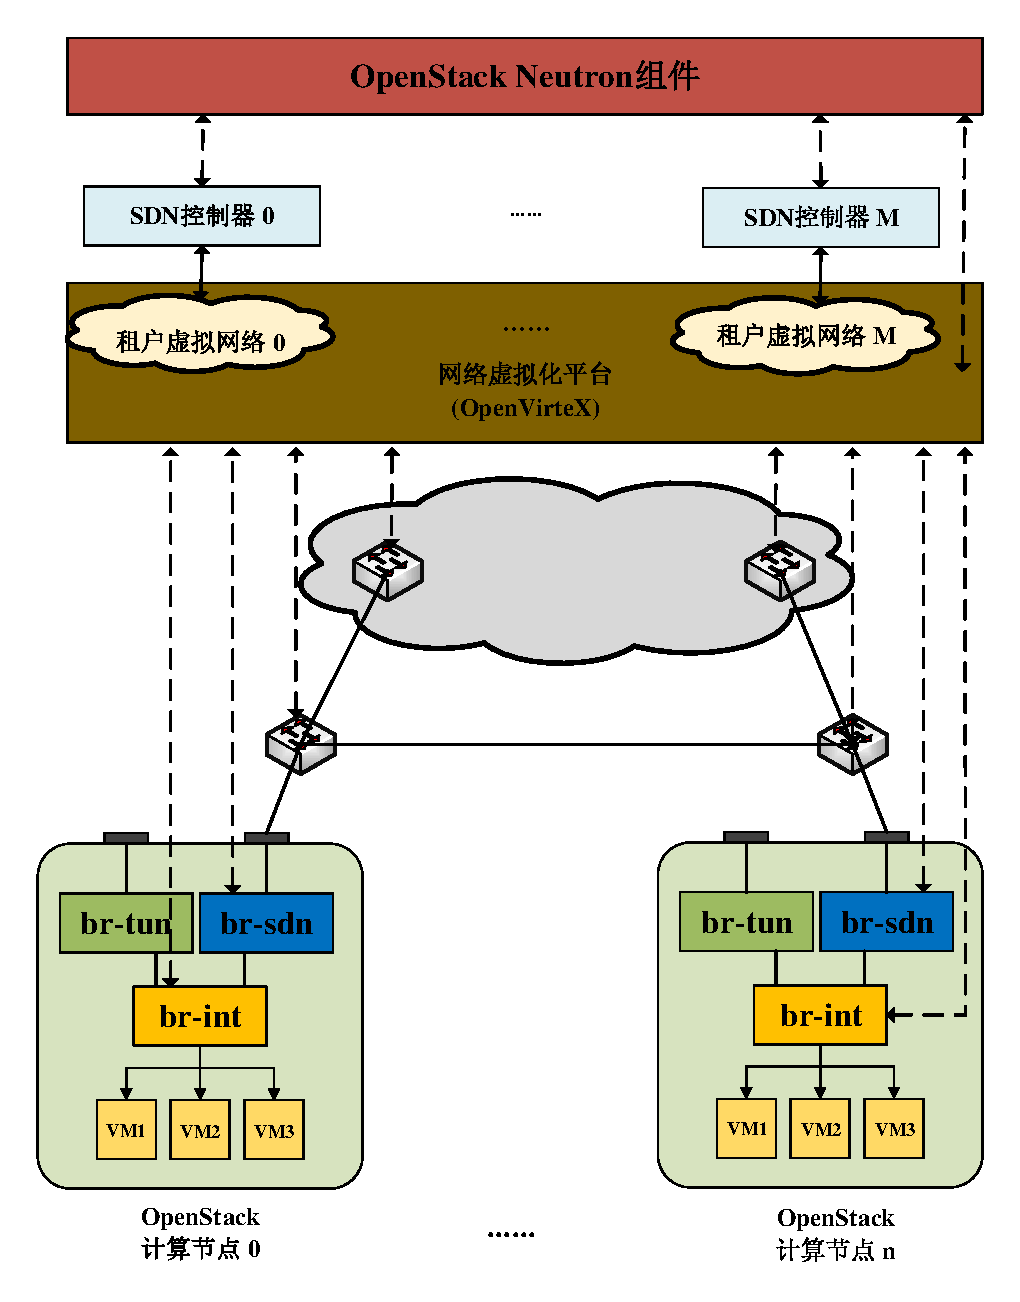
\includegraphics[width=120mm]{logo/architecture}\\
  \caption{System environment.}
  \label{fig:env1}
\end{figure}

%% 本章参考文献
\ifx\usechapbib\empty
\nocite{BSTcontrol}
\setcounter{NAT@ctr}{0}
\bibliographystyle{buptgraduatethesis}
\bibliography{bare_thesis}
\fi
